\graphicspath{{chapters/notes/04/images}}
\chapter{IGV (Integrative Genomics Viewer)} \label{chap: IGV}

\section{IGV characteristics}

    \subsection{Introduction}
    The human genome nowadays is being explored extensively thanks to:

    \begin{multicols}{2}
        \begin{itemize}
            \item Exons and whole-genome sequencing.
            \item Epigenetic surveys.
            \item Expression profiling of coding and noncoding RNAs.
            \item SNPs and copy number profiling.
            \item Functional assays.
        \end{itemize}
    \end{multicols}

    IGV allow to visually explore the data generated from this kind of study, which is mostly used for the development of precision medicine, an approach for disease treatment and prevention that takes into account individual variability in:

    \begin{multicols}{3}
        \begin{itemize}
            \item Genes.
            \item Living environment.
            \item Lifestyle.
        \end{itemize}
    \end{multicols}

    The objective of precision medicine is to define which drug, at what time and at what dose to administer to an ill individual to have optimal response.
    The IGV software is a high-performance lightweight visualization tool for interactive exploration of large, integrated genomic datasets.
    It supports a wide variety of data types, including next-generation sequence data, and genomic annotations.
    Data sets can be loaded from local or remote sources, including cloud-based resources.
    In IGV, each vertical bar corresponds to a read.
    A coloured sign in a read indicates the presence of a polymorphism.
    The browser also gives info about the quality of the read and the bases from the loaded BAM file.
    Other information regarding IGV are present in the \href{https://authors.library.caltech.edu/72234/2/nbt.1754-S1.pdf}{Supplementaty information - Integrative Genomics Viewer} pdf file.

    \subsection{Main uses of IGV}
    Some utilization of IGV are:

    \begin{multicols}{2}
        \begin{itemize}
            \item NGS alignment.
            \item Epigenomics studies.
            \item Copy number evaluations.
            \item RNA-sequencing.
            \item Identification of variants and genotypes.
        \end{itemize}
    \end{multicols}

    Some of the main utilization are represented in figure \ref{fig:IGVusages}.

    \begin{figure}[H]
        \centering
        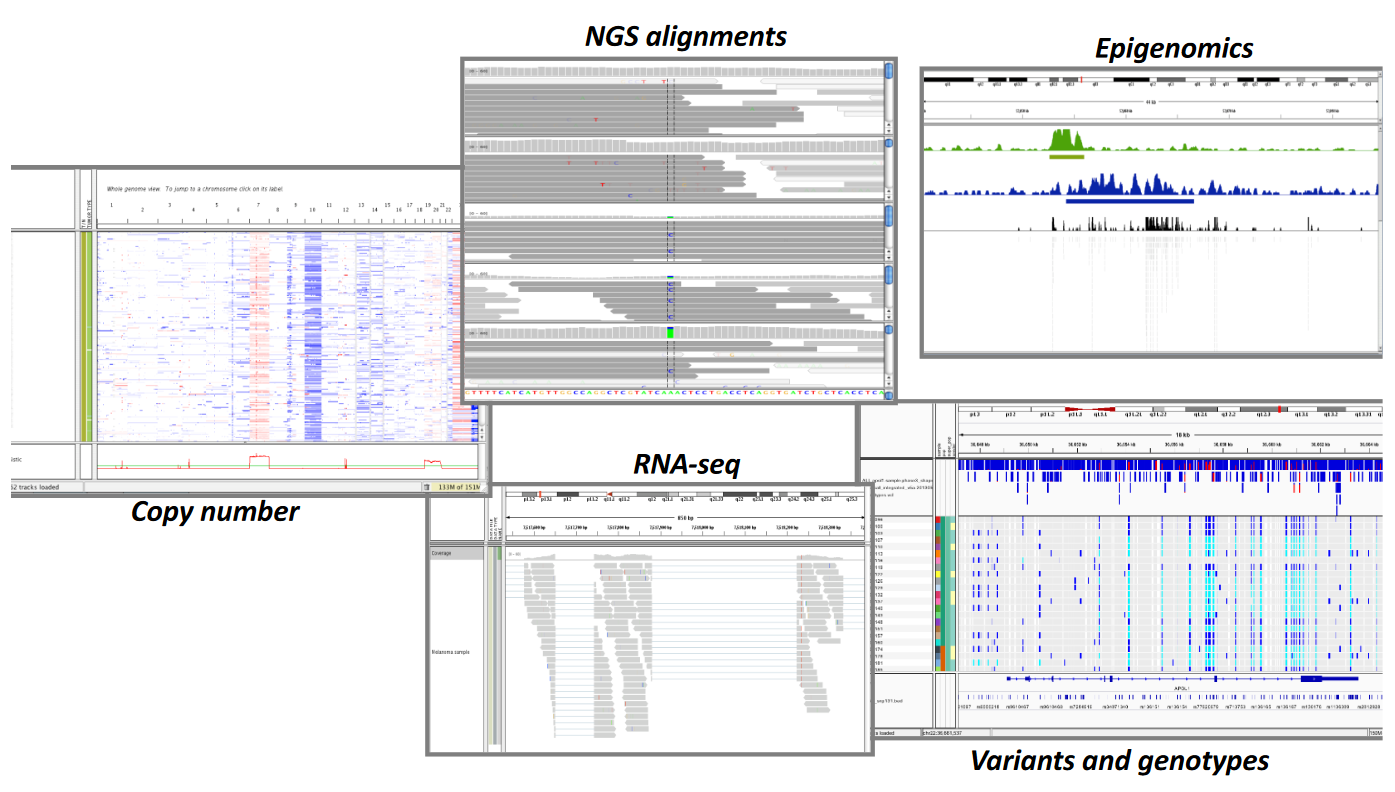
\includegraphics[width=0.8\textwidth]{usagesIGV.PNG}
        \caption{Main type of data exploration done with IGV.}
        \label{fig:IGVusages}
    \end{figure}

        \subsubsection{RNA sequence analysis}
        IGV can be used to explore RNA sequence analysis.
        For example figure \ref{fig:RNAseq} represents reads that span exon junctions, with their heights depending on the number of reads that connect them.

        \begin{figure}[H]
            \centering
            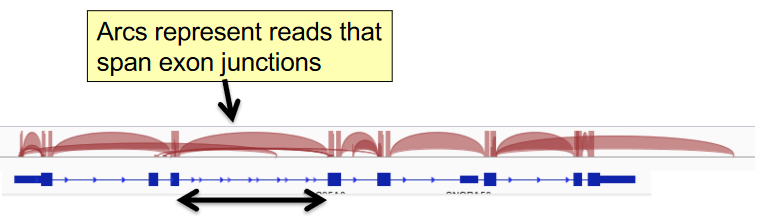
\includegraphics[width=0.7\textwidth]{RNAseqAlign.PNG}
            \caption{View of RNA sequence data for a gene.}
            \label{fig:RNAseq}
        \end{figure}

        Another thing that can be done are Sashami plots.
        In these plots the number of reads connecting exosomes are represented on curved lines.
        The peaks represents coverage within exons.
        An example of a Sashami plot is depicted in figure \ref{fig:sashami}.

        \begin{figure}[H]
            \centering
            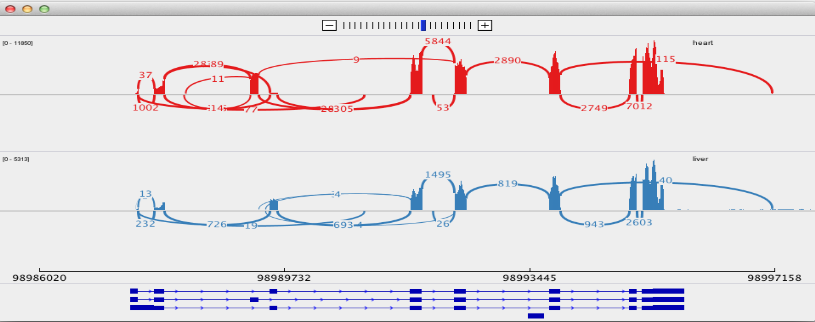
\includegraphics[width=0.8\textwidth]{sashamiplot.PNG}
            \caption{Sashami plots}
            \label{fig:sashami}
        \end{figure}

        \subsubsection{Variant discovery}
        IGV allows to study variants from different samples, like it can be seen in figure \ref{fig:variants}

        \begin{figure}[H]
            \centering
            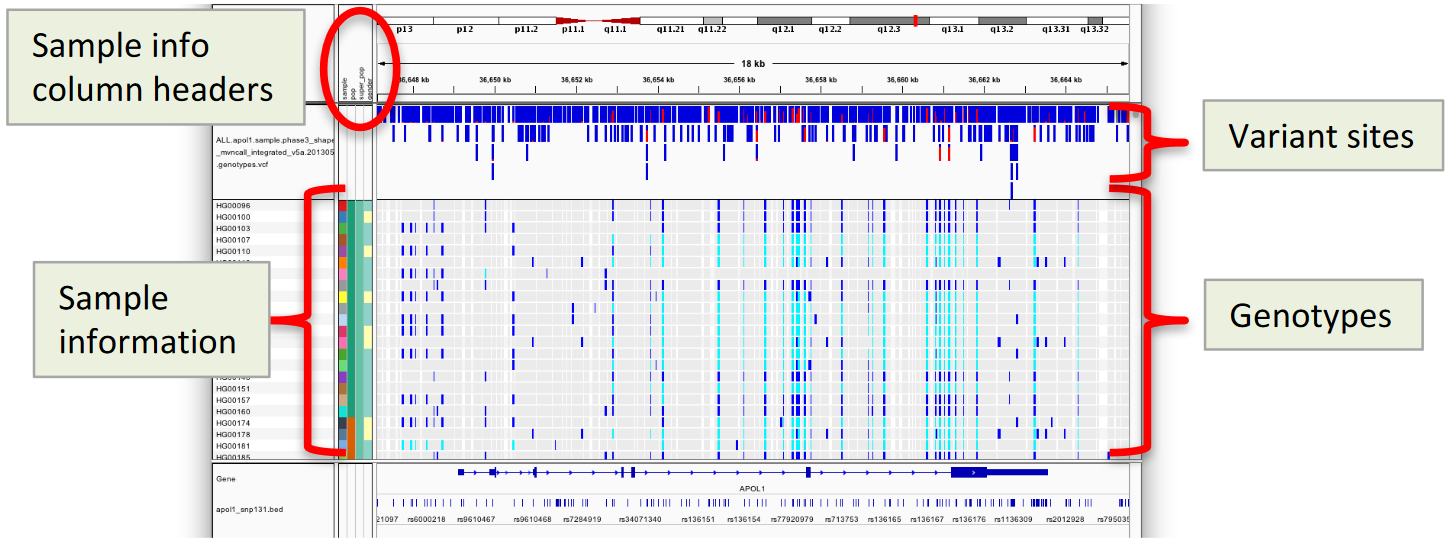
\includegraphics[width=0.9\textwidth]{variantsView.PNG}
            \label{fig:variants}
        \end{figure}

    \subsection{Operations}
    IGV allows for the simultaneous visualization of an arbitrary number of BAM files.
    The user can move, zoom in and out quickly over different genomic scales, panel \emph{a} of figure \ref{fig:IGV_navigation}), and also to jump in precise positions of the sequence.
    It is possible to search for genomic coordinates or gene names.
    For each resolution scale called zoom levels, the aggregated data is divided into tiles, panel \emph{b} of figure \ref{fig:IGV_navigation}) that correspond to a region viewable on a typical user display.
    Each tile is subdivided into bins, with the width of a bin chosen to correspond to the width represented by a pixel at that resolution scale.
    It is also possible to sort the samples in different ways and to group them considering different characteristics.


    \begin{figure}[H]
        \begin{tabular}{cc}
          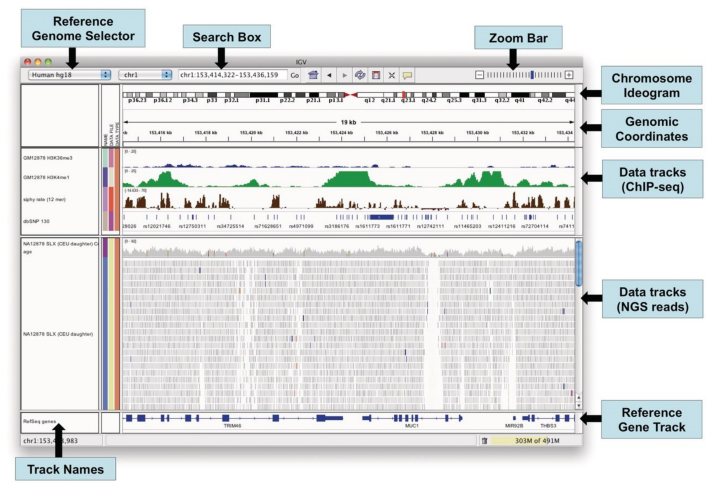
\includegraphics[width=0.5\textwidth]{IGVview.PNG} &   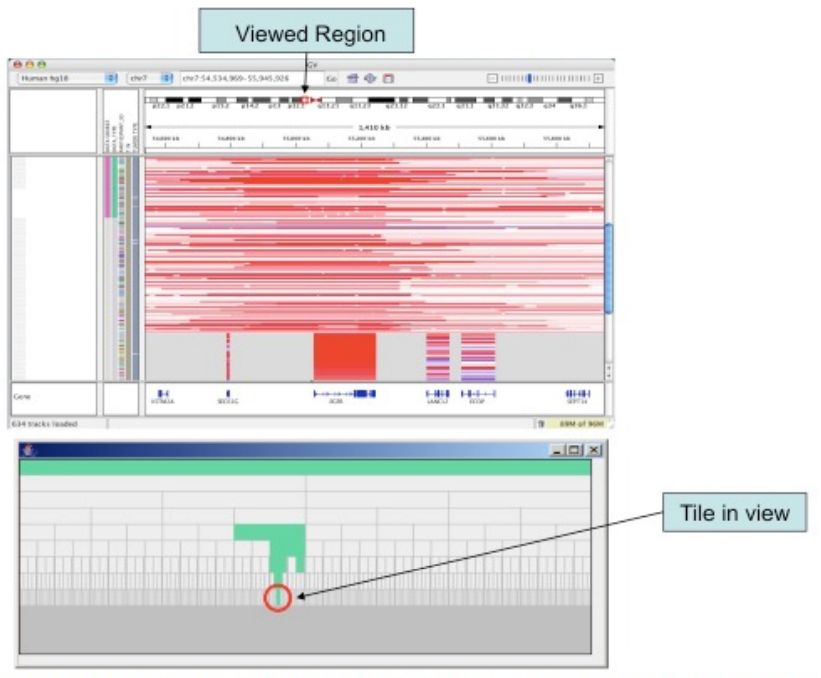
\includegraphics[width=0.5\textwidth]{TileView.PNG} \\
        (a) IGV interface main features & (b) Tiles view in IGV \\[6pt]
        \end{tabular}
        \caption{}
        \label{fig:IGV_navigation}
    \end{figure}

    Navigation through a data set is similar to that of \textit{Google Maps}, allowing the user to zoom and pan seamlessly across the genome at any level of detail from whole genome to base pair.
    Annotations for specific genomes could be found consulting the UCSC Table Browser \href{http://genome.ucsc.edu/cgi-bin/hgTables}{(UCSC table)}.\\

    \subsection{Tiles}
    The corresponding data tiles for each zoom level are stored in the binary Tiled Data Format, or TDF, which has been optimized for fast tile retrieval.
    A tiled data file (.tdf) is a binary file that contains data that has been preprocessed for faster display in IGV.
    TDF files are generated by using the \textit{igvtools} package (\textit{toTDF} command).
    Tile sizes for each zoom level are constant and small.
    A single tile at the lowest resolution (spanning the entire genome) has the same memory footprint as a tile at the very high zoom levels (might span only a few kilobases).
    Tiles no longer in view are discarded as needed to free memory.

        \subsubsection{Pixel resolution error}
        Pixel resolution errors occur when data density exceeds the constraint given by the number of pixels available for display.
        This can be solved through data aggregation.
        As the user zooms below the $\sim 50 kb$ range, individual aligned reads become visible, like in figure \ref{fig:ViewReads}.
        It is possible then to zoom further, and see the bases at each position.

        \subsubsection{Data displayed at different resolutions}

        \begin{figure}[H]
            \centering
            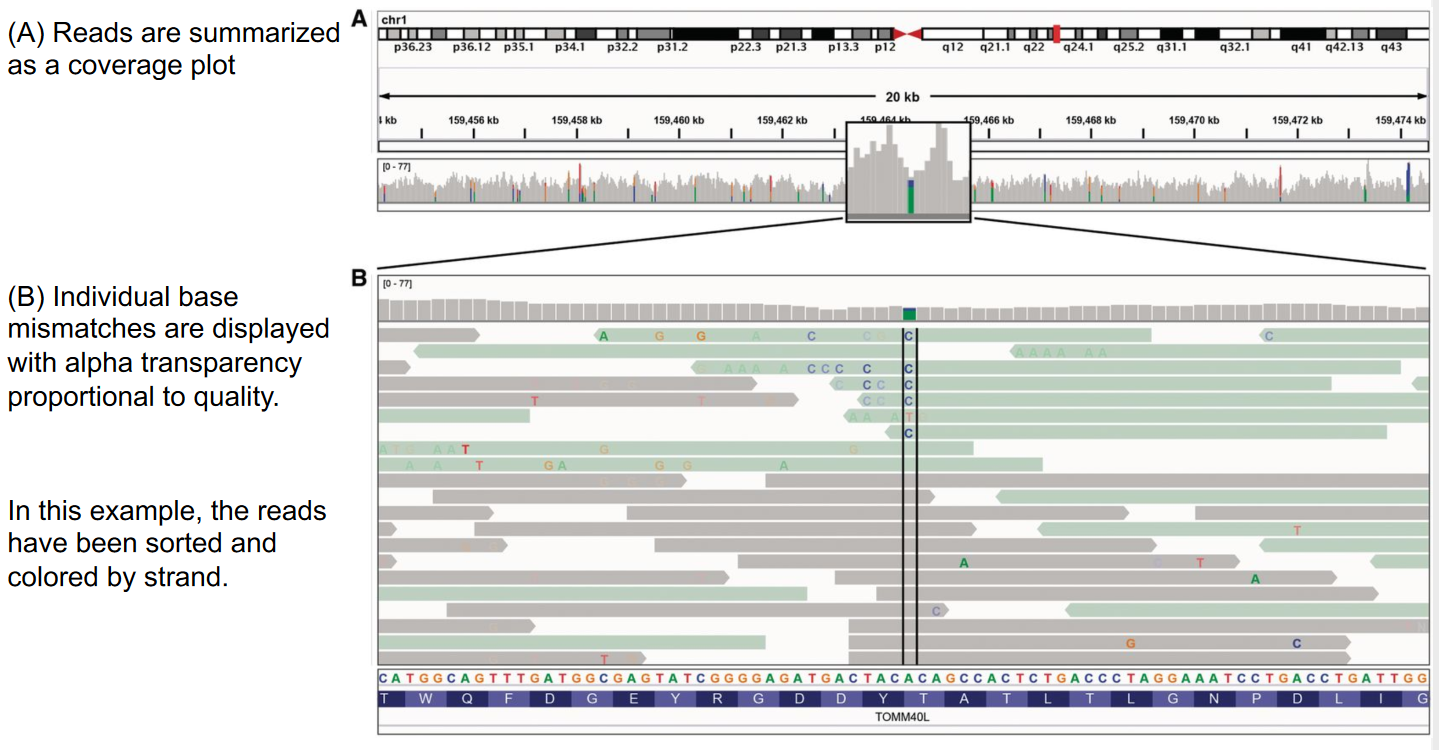
\includegraphics[width=0.7\textwidth]{IGVReadsView.PNG}
            \caption{Different resolution of IGV}
            \label{fig:ViewReads}
        \end{figure}

        In panel a of figure \ref{fig:ViewReads} reads are summarized as a coverage plot.
        In panel b individual base mismatches are displayed with alpha transparency proportional to quality.
        In this example, the reads have been sorted and coloured by strand and span a $20 kb$ genomic region for $1$ individual.
        The coverage is between $0$ and $77$ at certain positions there is more than one base supported by the reads.
        This is visualised by the green and blue column: some reads support $C$ instead of $A$.
        The coloured area is proportional to the allelic fraction for each base.

    \subsection{IGVTools}
    Igvtools comprises a set of utilities to prepare large files for efficient display.
    Some commands are reported in figure \ref{fig:commands}.
    In particular the count function takes as input a BAM file to generate coverage data.
    The obtained file could be then loaded with the "Load pre-computed coverage data" command for faster loading times.

    \begin{figure}[H]
        \centering
        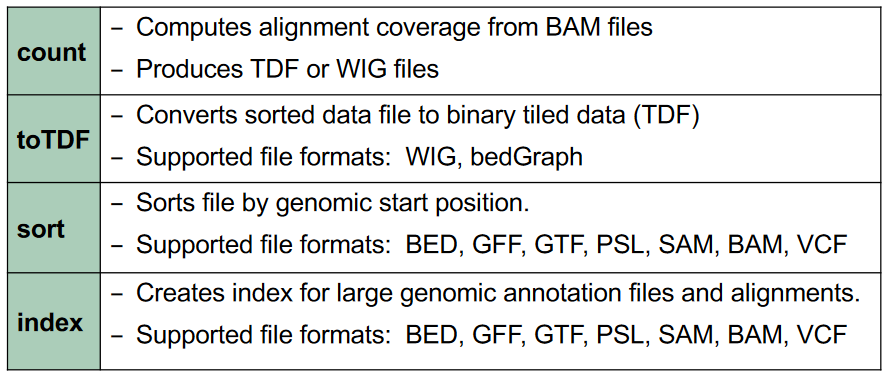
\includegraphics[width=0.6\textwidth]{igvtools.PNG}
        \caption{igvtools possible operations.}
        \label{fig:commands}
    \end{figure}

    \subsection{Session files}
    Sessions allow users to share their data and views with other users simply and accurately.
    Session files describe the session state in XML.

\section{Interpreting pair orientations}
IGV allows to discover  genetic aberrations through the interpretation of pair orientation.
A paired end protocol can uncover:

\begin{multicols}{3}
    \begin{itemize}
        \item Inversions.
        \item Duplications.
        \item Translocations.
    \end{itemize}
\end{multicols}

To detect these kind of events reads that span the breakpoint are needed.
This type of reads can be obtained through long reads or paired-end sequencing.

    \subsection{Element to consider when interpreting pair orientations}
    Different parameters are to be considered when interpreting pair orientations:

    \begin{multicols}{2}
        \begin{itemize}
            \item Pair ends relative orientation.
            \item Insert size length.
            \item Coverage within the aberrant region.
            \item Coverage outside of the aberrant region (flanking genomic segments).
            \item Coverage at the breakpoints.
        \end{itemize}
    \end{multicols}

    In particular when considering pair ends relative orientation some considerations can be done:

    \begin{multicols}{2}
        \begin{itemize}
            \item \textbf{LR} ($\rightarrow\cdots\leftarrow$): is an Illumina convention, and implies that the reads are left and right of the unsequenced part of the sequenced DNA fragment when aligned back to the reference genome.
            \item \textbf{LL}, \textbf{RR} ($\leftarrow\cdots\leftarrow\land\rightarrow\cdots\rightarrow$): implies an inversion in sequenced DNA with respect to the reference.
            \item \textbf{RL} ($\leftarrow\cdots\rightarrow$): implies a duplication or translocation with respect to the reference.
        \end{itemize}
    \end{multicols}

    \subsection{Inversion}
    Figure \ref{fig:inversion} depicts an inversion.
    A local drop in coverage and reads direction $LL$ or $RR$ can be observed.
    Moreover a drop on the breakpoint can be observed.

    \begin{figure}[H]
        \begin{tabular}{cc}
            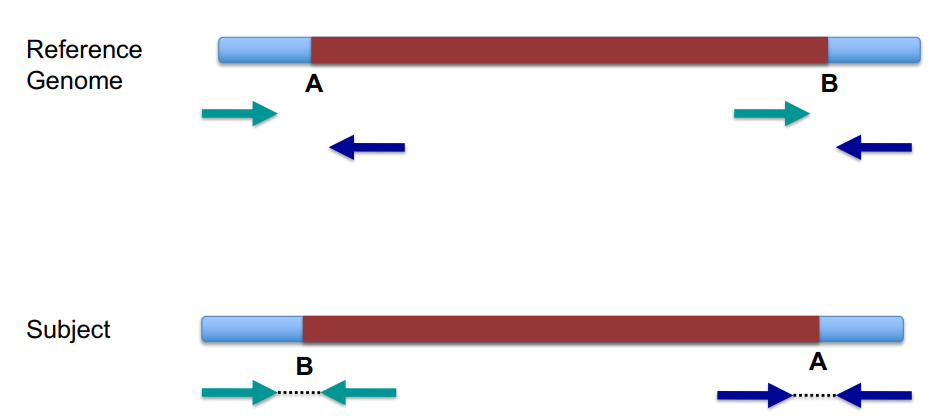
\includegraphics[width=0.5\textwidth]{inversion.png} &   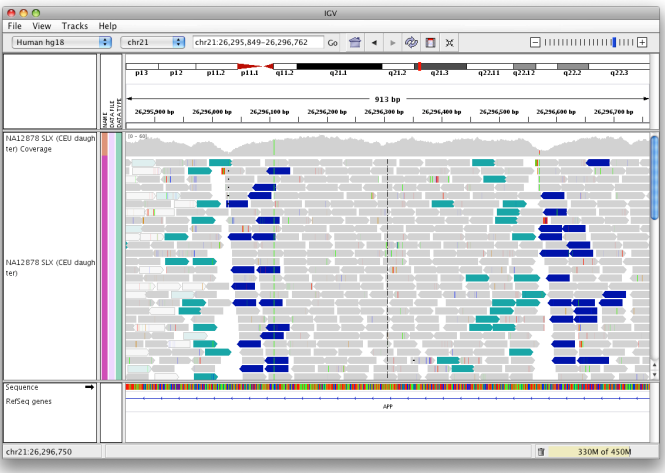
\includegraphics[width=0.5\textwidth]{inversion_igv.png} \\
            (a) Schematic & (b) IGV view \\[6pt]
        \end{tabular}
        \caption{Inversion discovering exploiting PE reads.}
        \label{fig:inversion}
    \end{figure}

    \subsection{Tandem duplication}
    Figure \ref{fig:tandem} depicts a tandem duplication.
    All the reads that do not cover the junction point align perfectly to the reference.
    Moreover it can be observed a $50\%$ increase of coverage proportional to the extra copy.
    Junctions $A$ and $B$ are not modified.
    A read mapping $BA$ would be partially aligned at $B$ on the reference.
    There is no drop in coverage.


    \begin{figure}[H]
        \begin{tabular}{cc}
            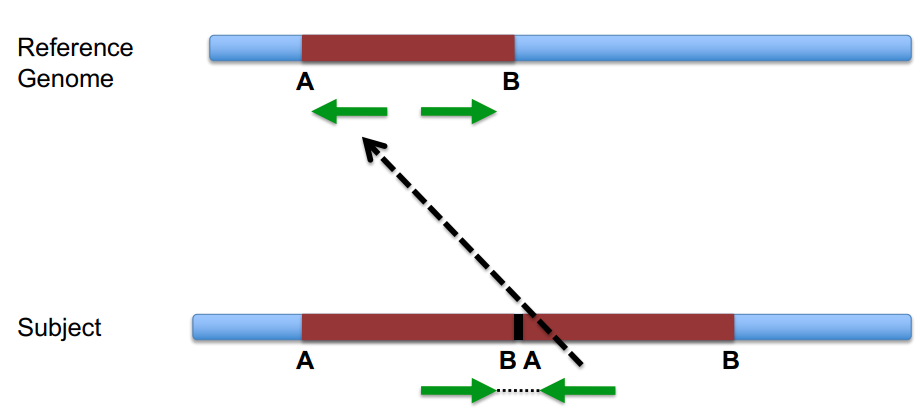
\includegraphics[width=0.5\textwidth]{tandem.png} &   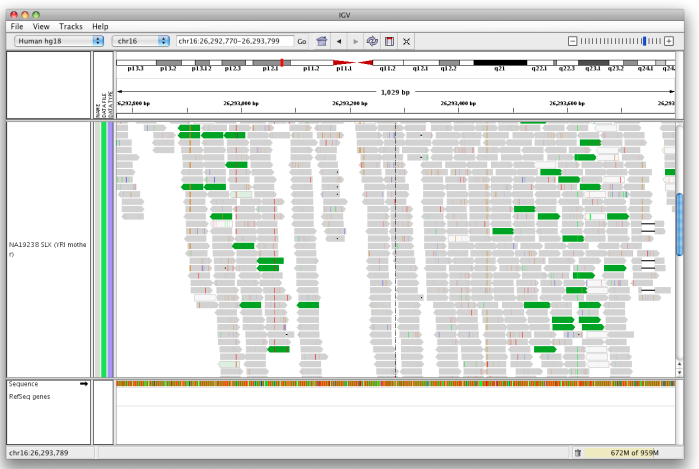
\includegraphics[width=0.5\textwidth]{tandem_igv.png} \\
            (a) Schematic & (b) IGV view \\[6pt]
        \end{tabular}
        \caption{Tandem duplication discovering exploiting PE reads.}
        \label{fig:tandem}
    \end{figure}

    \subsection{Inverted duplication}
    Figure \ref{fig:inverted} depicts an inverted duplication.
    Coverage increase in the duplicated site in the reference gene is expected.
    Both $A$ and $B$ on the first segment are $LR$, while the second will have reads oriented $LL$ or $RR$.
    The insert size will be significantly longer.
    An overlapping of left and right reads can be found on the reference.

    \begin{figure}[H]
        \begin{tabular}{cc}
            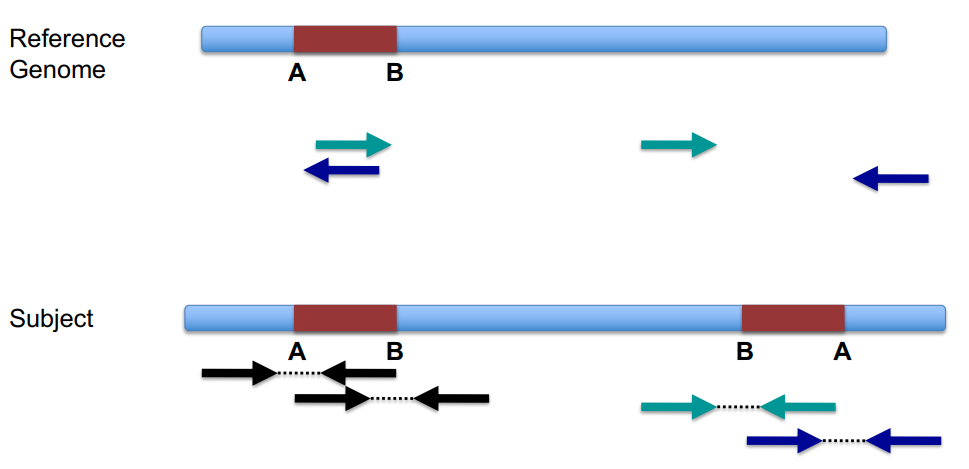
\includegraphics[width=0.5\textwidth]{inverted.png} &   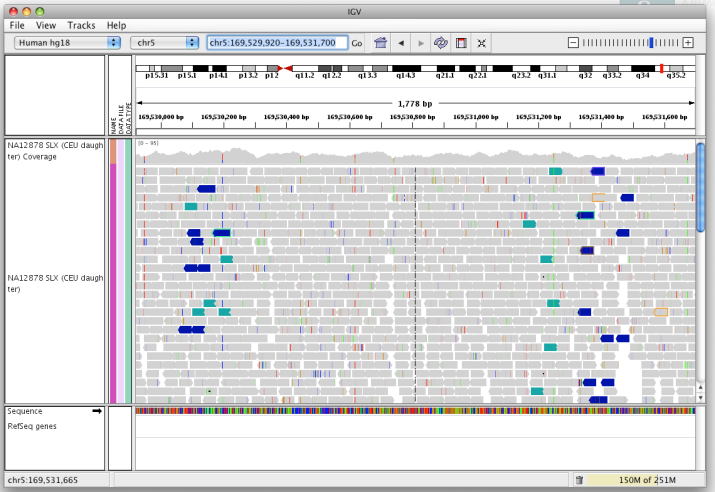
\includegraphics[width=0.5\textwidth]{inverted_igv.png} \\
            (a) Schematic & (b) IGV view \\[6pt]
        \end{tabular}
        \caption{Inverted duplication discovering exploiting PE reads.}
        \label{fig:inverted}
    \end{figure}

    \subsection{Deletion}
    Deletion can be discovered by observing drop in coverage or the observed distance between reads, which gives a clean indication of the size of the deletion.
    For small deletions like indels the sequence within the reads has to be observed.

\section{Uncovering genetic aberrations - some examples}

    \subsection{First example}
    Figure \ref{fig:task_a} depicts the genomic region chr1:11,050,009-11,055,137.
    The event visualized could be a tandem duplication on one of the two alleles and a deletion on the other allele.
    This is due to the fact that despite of the duplication the coverage on remains constant on the region.

    \begin{figure}[H]
        \centering
        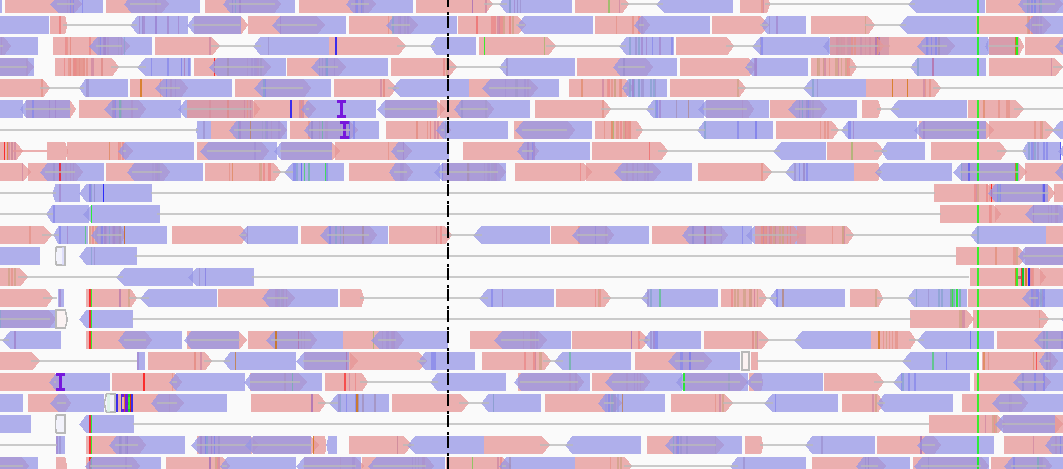
\includegraphics[width=0.8\textwidth]{pos1.PNG}
        \caption{A tandem duplication followed by a deletion}
        \label{fig:task_a}
    \end{figure}

    \subsection{Second example}
    Figure \ref{fig:task_b} depicts the genomic region chr5:9,410,315-9,413,699.
    It is clear due to the absence of coverage how both allele of that region were deleted.

    \begin{figure}[H]
        \centering
        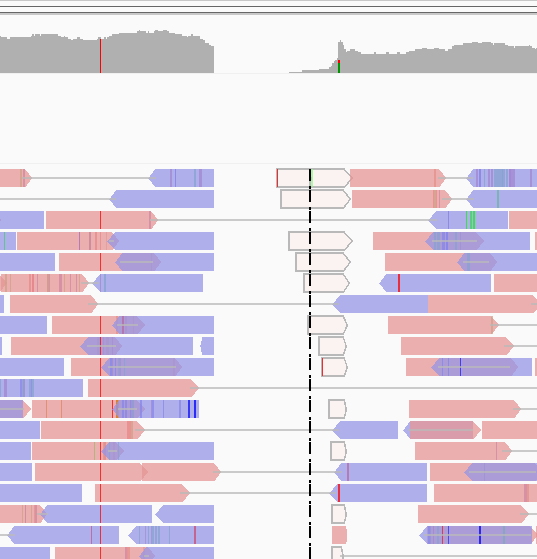
\includegraphics[width=0.6\textwidth]{pos2.PNG}
        \caption{An homozygous deletion}
         \label{fig:task_b}
    \end{figure}

    \subsection{Third example}
    Figure \ref{fig:cov3} and \ref{fig:ex_3} depicts an inverted duplication followed by a deletion.
    This prediction is justified because of the presence of overlapping $LR$ reads and $LL$ and $RR$ reads with a correspondent increase of coverage, followed in the following region by a considerable drop in coverage, indicating an heterozygous deletion.

    \begin{figure}[H]
       \centering
       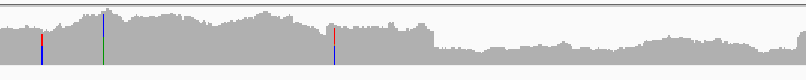
\includegraphics[width=1\textwidth]{cov3.PNG}
       \caption{Coverage for an inverted duplication followed by a deletion}
       \label{fig:cov3}
    \end{figure}


    \begin{figure}[H]
        \begin{tabular}{cc}
        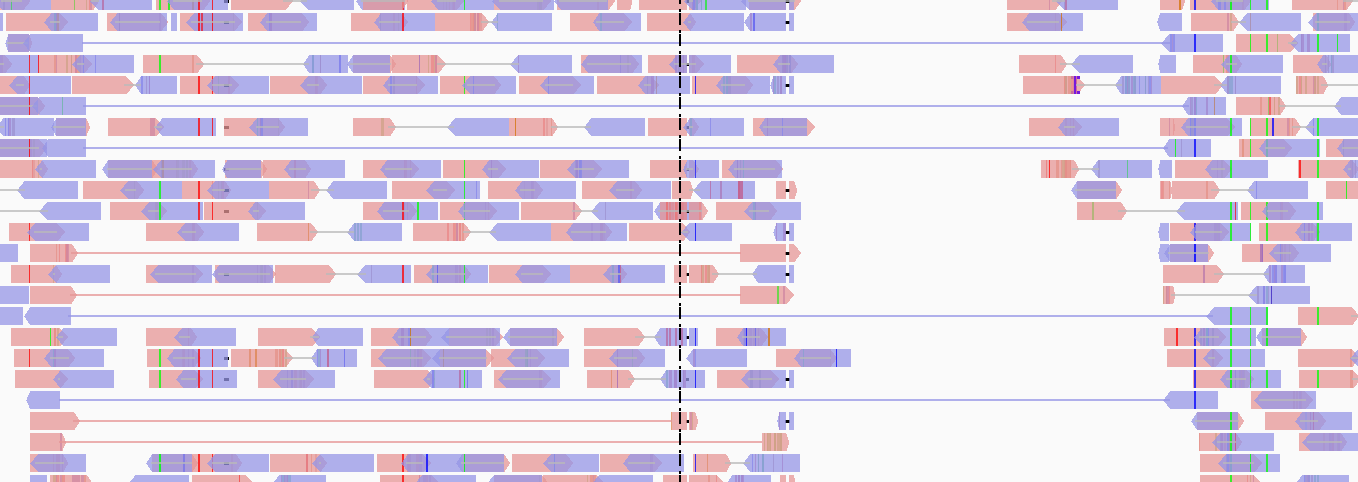
\includegraphics[width=0.5\textwidth]{pos3.PNG} &   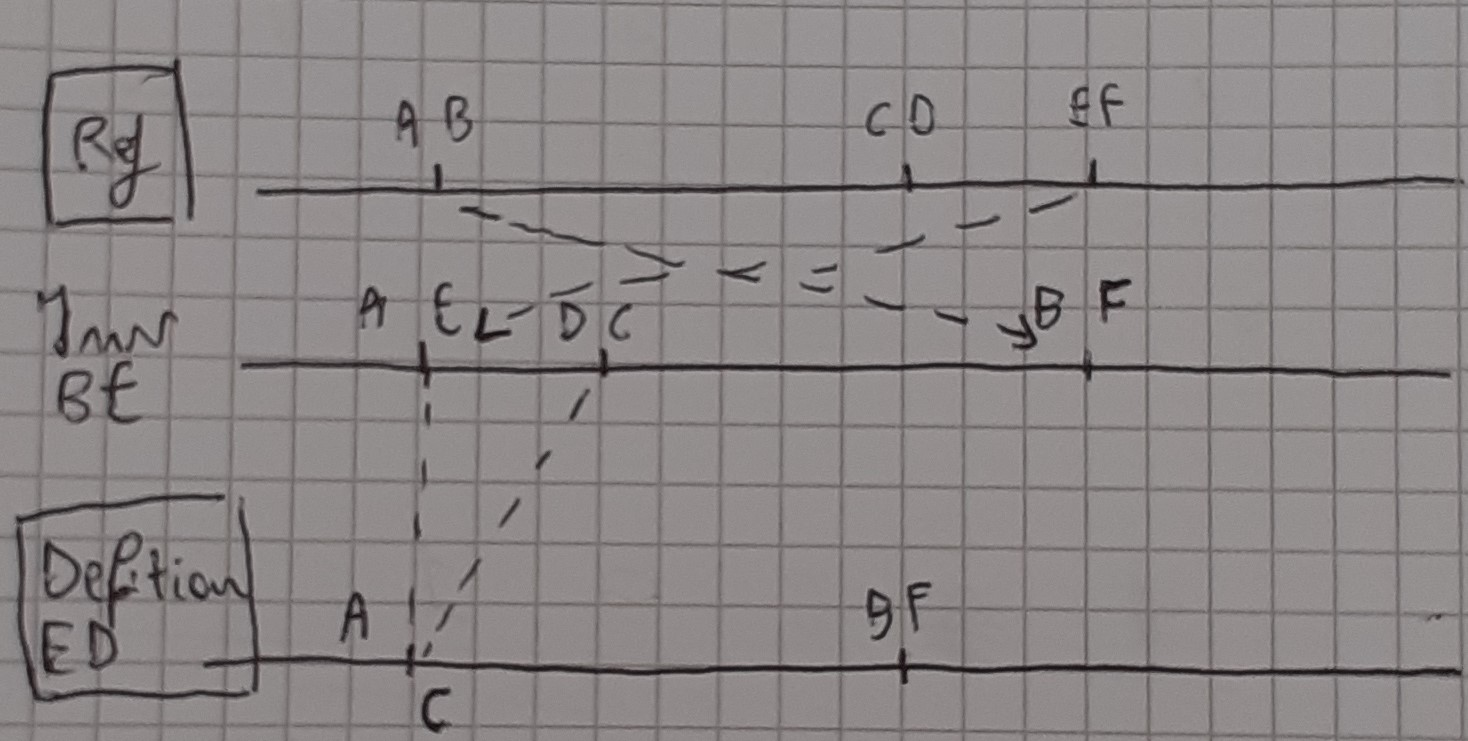
\includegraphics[width=0.5\textwidth]{pos3passages.jpg} \\
        (a) IGV view & (b) written passages \\[6pt]
        \end{tabular}
        \caption{Coverage for an inverted duplication followed by a deletion}
        \label{fig:ex_3}
    \end{figure}
